\documentclass[11pt]{article}

\usepackage{amsmath}
\usepackage{amssymb}
\usepackage{color}
\usepackage{listings}
\usepackage{graphicx}

\textwidth=6.5in
\textheight=9in
\topmargin=-0.8in
\headheight=15.75pt
\headsep=.35in
\oddsidemargin=0.0in
\evensidemargin=0.0in

\newcommand{\Complex}{\mathbb{C}}
\newcommand{\Real}{\mathbb{R}}
\newcommand{\Dpt}{D_{+t}}
\newcommand{\Dmt}{D_{-t}}
\newcommand{\Dzt}{D_{0t}}
\newcommand{\Dpx}{D_{+x}}
\newcommand{\Dmx}{D_{-x}}
\newcommand{\Dzx}{D_{0x}}
\newcommand{\vnpj}{v^{n+1}_j}
\newcommand{\vnjp}{v^n_{j+1}}
\newcommand{\vnjm}{v^n_{j-1}}

\begin{document}
\begin{flushright}
\small{MATH-6840\\
Vignesh Ramakrishnan\\
{\bf Due: Monday January 31, 2022}}
\end{flushright}

\begin{center}
\large{Problem Set 2}\\
\end{center}


\begin{enumerate}
  %%%%%
  %%%%%
  %%%%%
  \item (15 pts.) {\em Adopted from NPDE exercise 1.2.1:}\\
  {\color{red}Write a code to approximately solve }
  \begin{align*}
    v_t & = \nu v_{xx}, \qquad x\in(0,1), \qquad t>0\\
    v(x,0) & = f(x), \qquad x\in(0,1)\\
    v(0,t) & = a(t), \qquad v(1,t) = b(t), \qquad t\ge 0.
  \end{align*}
  {\color{red} Use the grid} $x_j=j\Delta x$, {\color{red} with} $j=1,2,\ldots,N$, {\color{red}  and} $\Delta x = 1/N$ {\color{red} (as described in the text), and apply the usual second-order centered spatial discretization with forward Euler time integration, i.e.}
  \begin{align*}
    \Dpt v_j^n = \nu\Dpx\Dmx v_j^n.
  \end{align*}
 { \color{red}Use }$f(x) = \sin(2\pi x)$, $a=b=0$, $\nu=1/6$, {\color{red} and} $N=10$. {\color{red} Find solutions at }$t=0.06$, $t=0.1$, $t=0.9$, {\color{red} and} $t=50.0$. {\color{red} For the first three values of} $t$,{\color{red} use} $\Delta t = 0.02$. {\color{red} To speed the solution to the last value of }$t$, {\color{red} you might use a larger value for} $\Delta t$. {\color{red} Determine how large you can choose} $\Delta t$ {\color{red} and still get results that might be correct. Compare and contrast your solution to the exact solution.}

The second-order centered spatial discretization with forward Euler time integration is given by the set of equations for all the nodes ranging from $j = 0,1,2,3 ..., N-1,N$:
\begin{align*}
D_{+t}v^n_j &= \nu D_{+x}D_{-x}v^n_j \\
v^{n+1}_j & = v^n_j + \frac{\nu \Delta t}{\Delta x^2}\left(v^n_{j+1} - 2v^n_j + v^n_{j-1}\right)
\end{align*}  
 One ghost node is added to the left side of the boundary node $x_j, \ j=0$ and it is called $x_{-1}$. Similarly one ghost node is added to the right side of the boundary node $x_j, \ j= N$ and it is named as $x_{N+1}$. Compatibility  boundary conditions are applied to figure out the values at these ghost nodes and this technique is used to apply the boundary conditions $v(0,t) = a(t)$, and $v(1,t) = b(t)$, $t\geq0$. 
 Compatibility boundary conditions specify that a time derivative is obtainable at both the boundary conditions and hence the following formulation comes about:
 \begin{align*}
v(0,t) & = a(t), \\
 v_t(0,t) & = a_t(t) \\
 \nu v_{xx}(0,t)&  = a_t(t) \\
 v^n_{-1} & = \frac{\Delta x^2}{\nu} a_t(t^n) + 2v^n_0 - v^n_1 \\
 \text{Similarly} & \\
 v^n_{N+1} & = \frac{\Delta x^2}{\nu} b_t(t^n) + 2v^n_{N} - v^n_{N-1}
 \end{align*}
 \lstinputlisting[language=Matlab, numbers=left, stepnumber=1, firstline=1,caption={Euler Forward-Step time marching - Heat Equation (Q.1)},label=code:myCode,frame=single]{HeatEqn1D.m}

The solutions at time $t = 0.06$, $t = 0.1$,  $t = 0.9$, and at $t = 50$ are displayed in Fig~\ref{fig:q1}. To speed up the solution, $\Delta t$ was raised from $0.02$ to $0.03$ and the solution still looked feasible. $\Delta t=0.03$ yields a CFL number $r = 0.5$ and if $\Delta t$ is increased to any value over $0.03$, CFL number, $r > 0.5$ and this makes the solution look implausible and at $t=50$, the values of the solutions blow up.
\begin{figure}[t]
\begin{tabular}{cc}
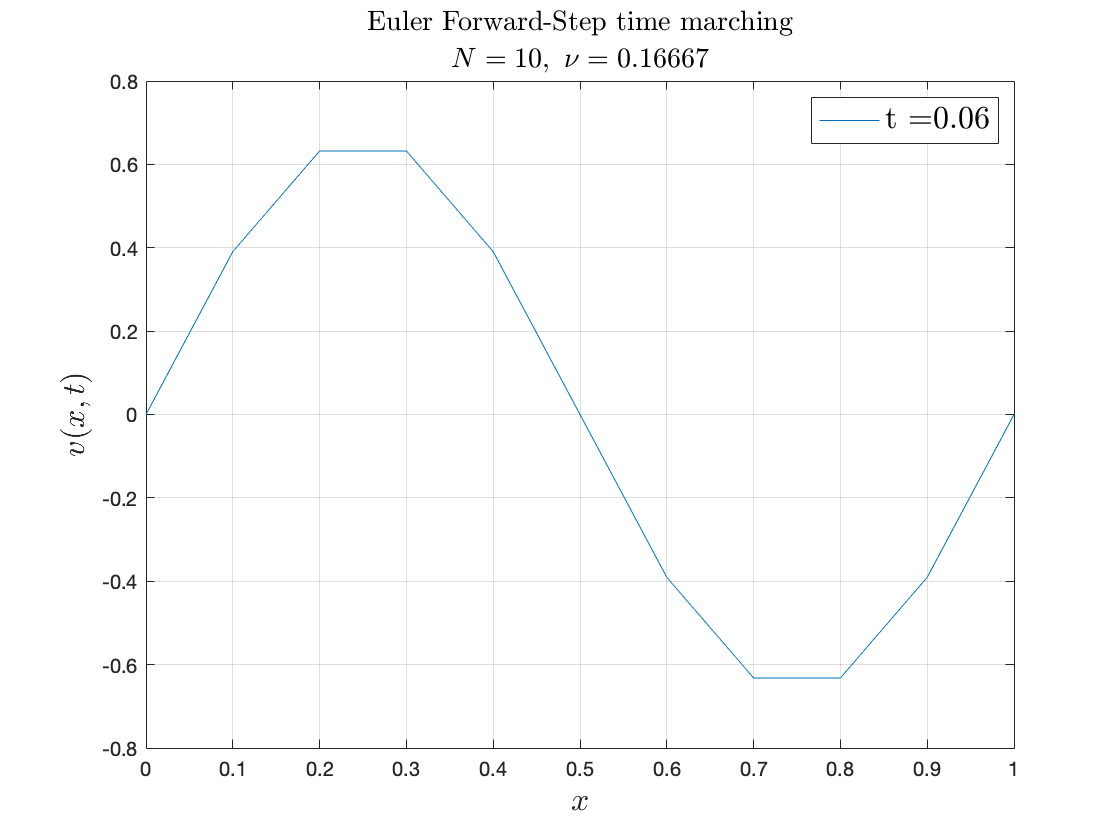
\includegraphics[width=3.65in]{q1_t1} & 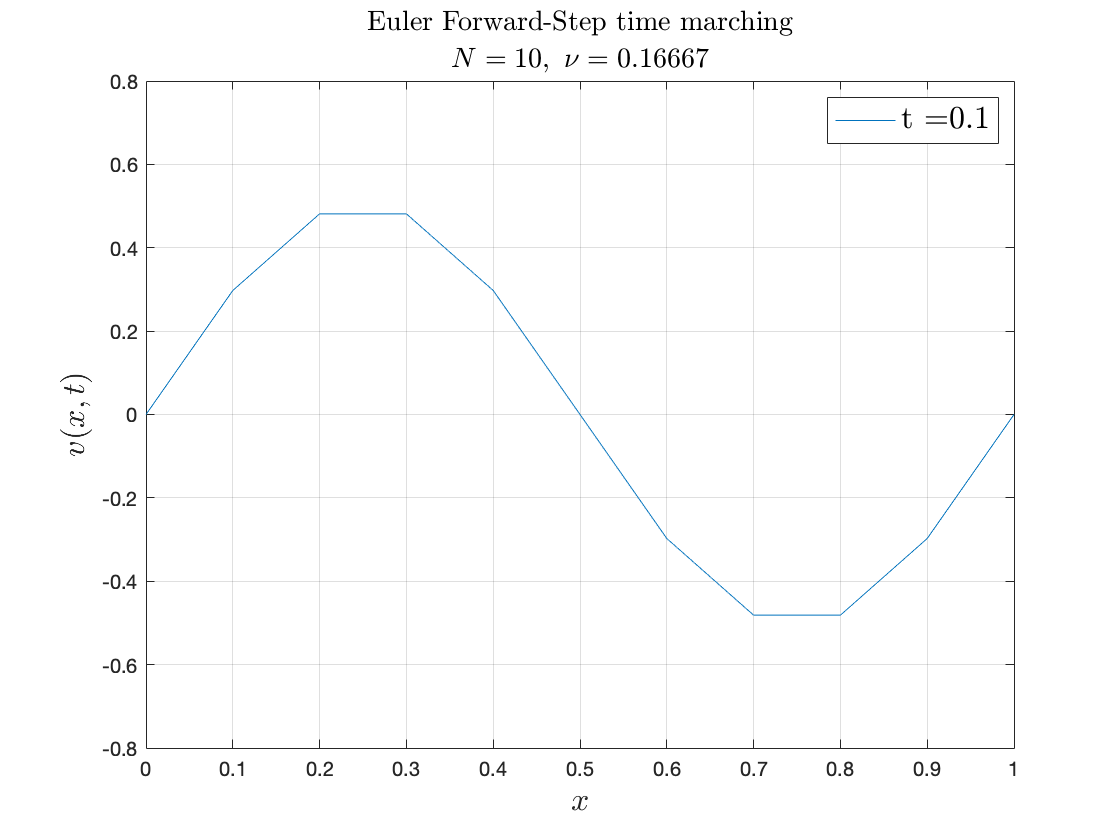
\includegraphics[width=3.65in]{q1_t2} \\
 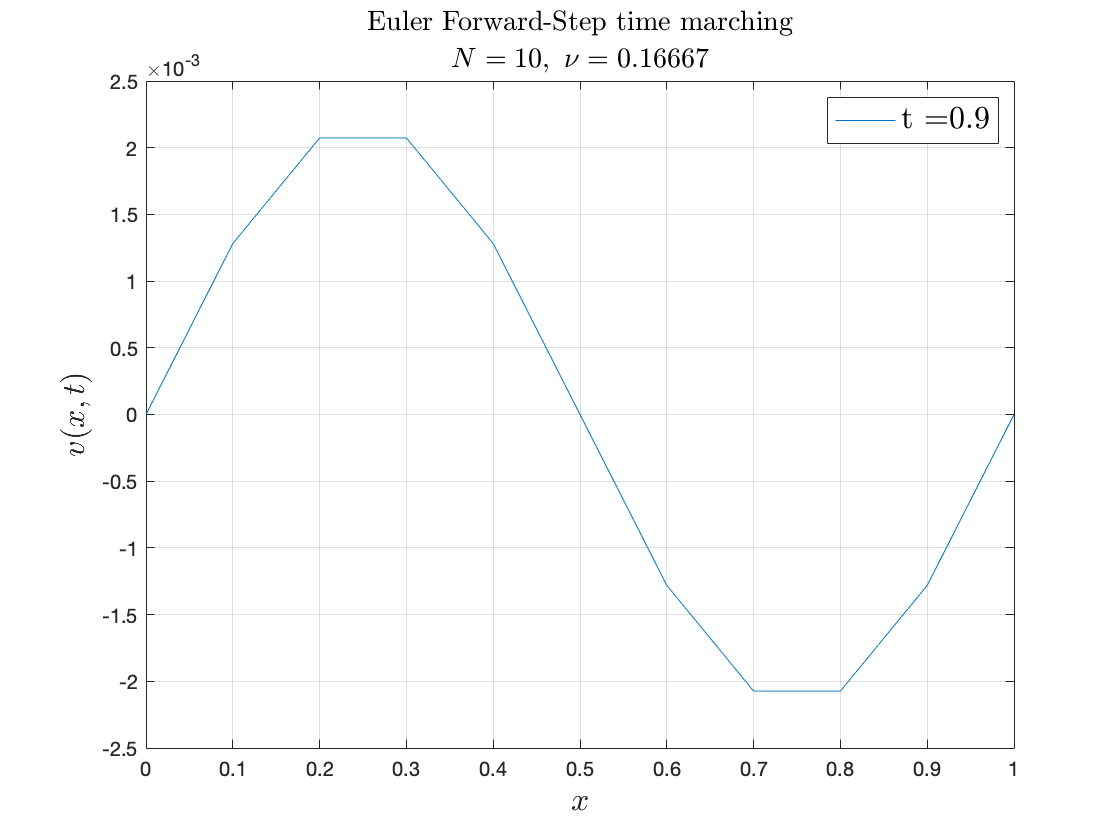
\includegraphics[width=3.65in]{q1_t3}  &  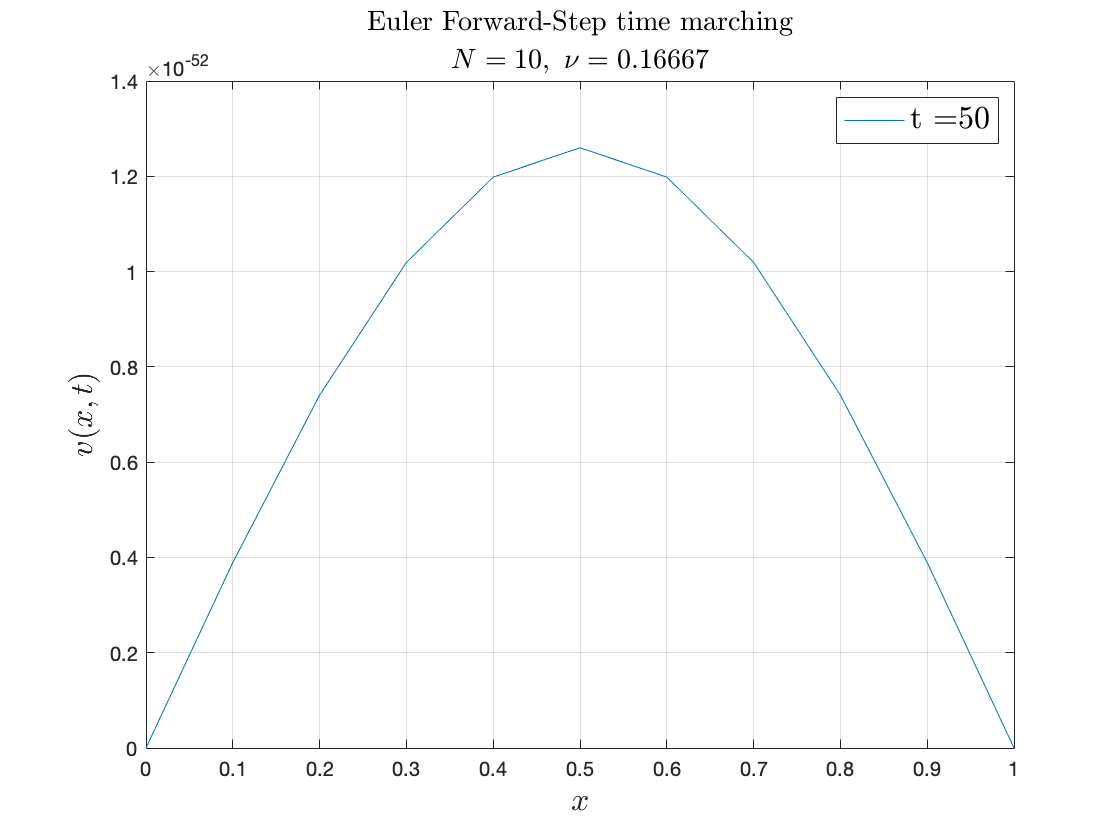
\includegraphics[width=3.65in]{q1_t4} \\
\end{tabular}
 \caption{Solution for $N = 10,\ \Delta t = 0.02$, at $t = 0.06, t=0.1, t=0.9, t=50$}
 \label{fig:q1}
 \end{figure}
  %%%%%
  %%%%%
  %%%%%
  \item (10 pts.) {\color{red}\em Adopted from NPDE exercise 1.3.1:}\\
  {\color{red}Solve the IBVP from problem (1) using leapfrog temporal integration, i.e.}
  \begin{align*}
    \Dzt v_j^n = \nu\Dpx\Dmx v_j^n.
  \end{align*}
  {\color{red}Recall that} $\Dzt v_j^n = \frac{1}{2}(\Dpt+\Dmt)v_j^n=\frac{v_j^{n+1}-v_j^{n-1}}{2\Delta t}$. {\color{red}For convenience, use the values form the exact solution at} $t=\Delta t$ {\color{red}to get the leapfrog scheme started. Do only the part with} $\Delta t=0.02$. {\color{red}It is also suggested that if the results of this problem are not nice, do note spend the rest of your life on in.}\\
To implement the leapfrog time scheme, it is important to know the solution at the second time-step along with the initial conditions. The exact solution to this PDE is found using the dispersion relationship.
\begin{align*}
v(x,t) & = \sin(2\pi x)e^{-4\pi^2 \nu t} \\
\text{Applying the differences,} \\
\vnpj & = v^{n-1}_j + \frac{2\nu \Delta t}{\Delta x^2}\left(\vnjp - 2v^n_j + \vnjm \right) \\
\vnpj & = v^{n-1}_j + 2r\left(\vnjp - 2v^n_j + \vnjm \right)
\end{align*}
For the solution at first time-step, $\Delta t = 0.02$, the solution is 
\begin{align*}
v(x,\Delta t) & = \sin(2\pi x)e^{-4\pi^2 \nu \Delta t}
\end{align*}
The code is attached for the leapfrog time-step method below. \\
 \lstinputlisting[language=Matlab, numbers=left, stepnumber=1, firstline=1,caption={Leap Frog time marching - Heat Equation (Q.2)},label=code:myCode,frame=single]{LeapFrog1D.m}
The solutions for this time marching approach is attached in Fig~\ref{fig:q2}. The solutions for $t=0.9$, and $t=50$ have blown up and are unstable. Hence, those plots have not been attached.
\begin{figure}[htp]
\begin{tabular}{cc}
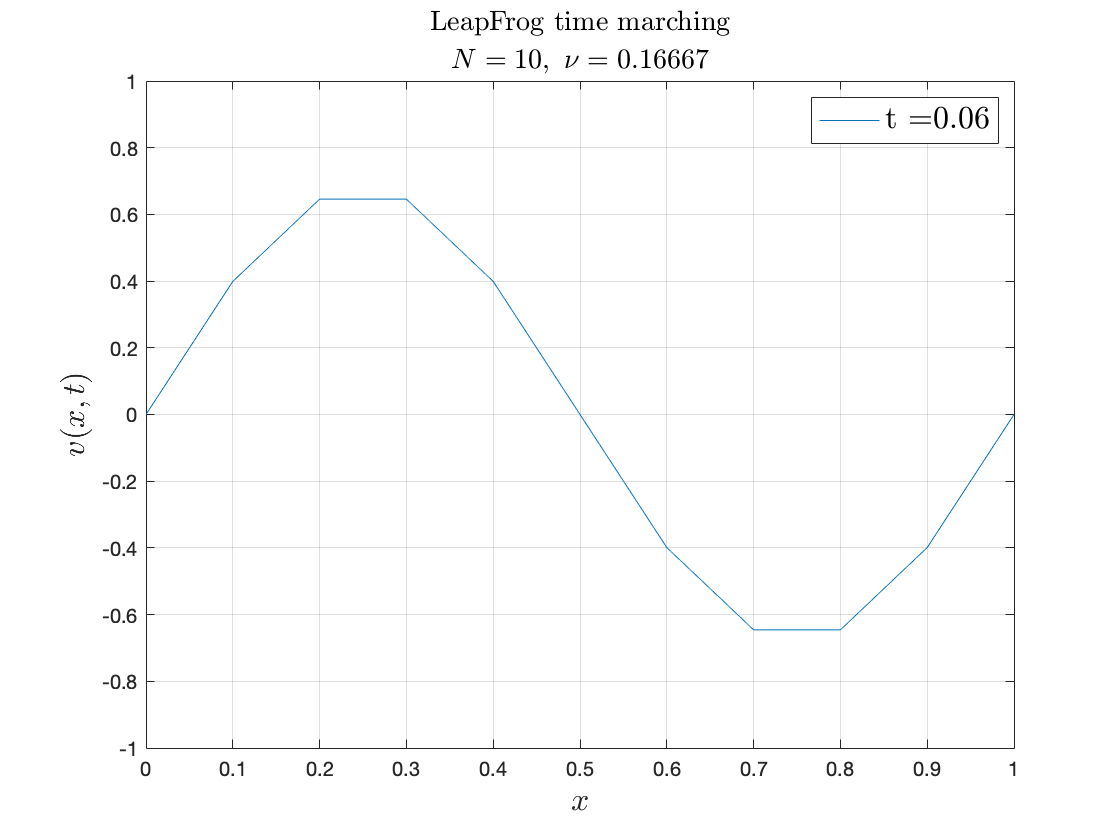
\includegraphics[width=3.65in]{q2_t1} & 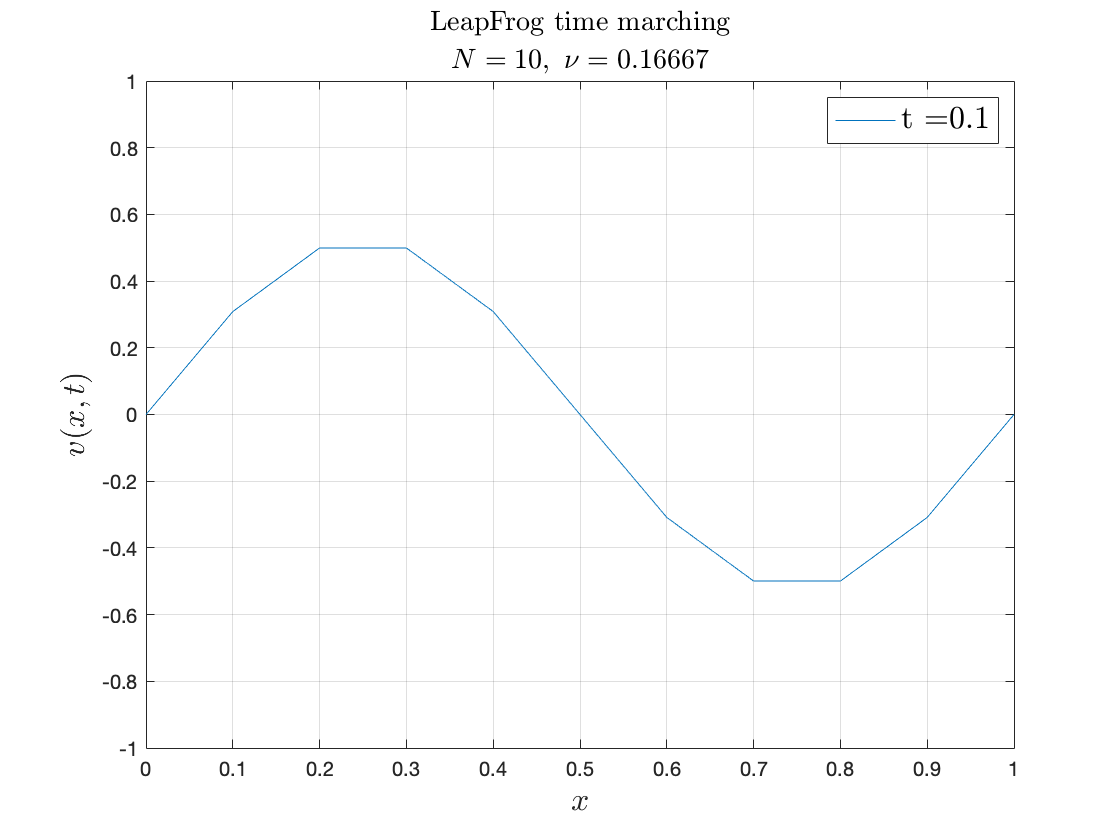
\includegraphics[width=3.65in]{q2_t2}
\end{tabular}
\caption{Solution for $N=10, \Delta t = 0.02$, at $t=0.06, t=0.1, t=0.9$, and $t=50$}
\label{fig:q2}
\end{figure}
  %%%%%
  %%%%%
  %%%%%
  \item (15 pts.)
  {\color{red}Consider the heat equation}
  \[
    u_t=\nu u_{xx}, \qquad x\in(0,1), \qquad t >0
  \]
  {\color{red}with initial conditions }
  \[
    u(x,t=0)=\sin\left(\frac{5\pi}{2}x\right),
  \] 
  {\color{red}and boundary conditions }
  \begin{align*}
    u(x=0,t) & = 0\\
    u_x(x=1,t) & = 0.
  \end{align*}
  %
  \begin{enumerate}
    \item {\color{blue}Write a code to solve this problem using the usual second-order centered spatial discretization with forward Euler time integration, i.e.}
  \begin{align*}
    \Dpt v_j^n = \nu\Dpx\Dmx v_j^n
  \end{align*}
  {\color{blue}on the grid defined by} $x_j=j\Delta x$, $j=0,1,\ldots,N$, $\Delta x=1/N$, {\color{blue}and the parameter }$r=\nu\Delta t/\Delta x^2=0.4$. {\color{blue}Ensure that your treatment of the boundary conditions are at least second-order accurate. Note that you may use a ghost cell to implement boundary conditions, but you are not required to do so. }\\
  
There is one Initial condition, one Dirichlet Boundary condition and one Neumann Boundary condition present for this PDE. It is well posed and the method to handle these boundary conditions is described below.
\begin{align}
u(x=0,t) & = 0 \\
u_x(x=1,t) & = 0
\end{align}
Two ghost node points are added, one to the left of the left boundary $(x_{-1})$ and one to the right of the right boundary $(x_{N+1})$.  Compatibility boundary condition is used for $(1)$ and a central difference approach on the last boundary node is computed to approximate $(2)$. 
\begin{align*}
v^n_{-1} & = 2v^n_0 - v^n_1 \\
v^n_{N+1} & = v^n_{N-1} \\
\vnpj & = v^n_j + r\left(\vnjp - 2v^n_j + \vnjm\right), \; j = 0,1,2,3,...,N-1,N \\
r & = \frac{\nu \Delta t}{\Delta x^2}
\end{align*}
The code is modified to accept CFL number, $r$ as an input and the time-step for time marching is calculated using $r$. Code is attached below in Listing 3. \\
 \lstinputlisting[language=Matlab, numbers=left, stepnumber=1, firstline=1,caption={Heat Equation (Q.3)},label=code:myCode,frame=single]{HeatEqn2_1D.m}

  \item {\color{blue}Setting} $\nu=1$, {\color{blue}perform a grid refinement study using} $N=20,40,80,160$ {\color{blue}by computing the maximum errors in the approximation at a final time} $t_f=.1$ {\color{blue}for grid points} $j=0,1,\ldots,N$ {\color{blue}(i.e. do not compute errors in ghost cells if you use them). Produce a }$\log$-$\log$ {\color{blue}plot showing the error as a function of} $\Delta x$, {\color{blue}and include a reference line indicating the expected rate of convergence.} \\
  
The code attached above was simulated at multiple suggested values of $N = 20,40,80,160$. The objective of this experiment is to verify the drop in the error between the actual solution and the numerical solution when the refinement of the spatial gird is increased. Actual solution is obtained using the dispersion analysis technique. The exact solution is given by:
\begin{align*}
u_{ex} & = \sin{\left(\frac{5\pi}{2}\right)}e^{-\frac{25\nu \pi^2 t}{4}} \\
e^n_j & = u^n_j - u_{ex}(x_j,t_n) 
\end{align*}
The maximum error among all the spatial points at final time $t_f = 0.1 \ \text{sec}$ is plotted in Fig~\ref{fig:q3b}.
\begin{figure}[htp]
\begin{center}
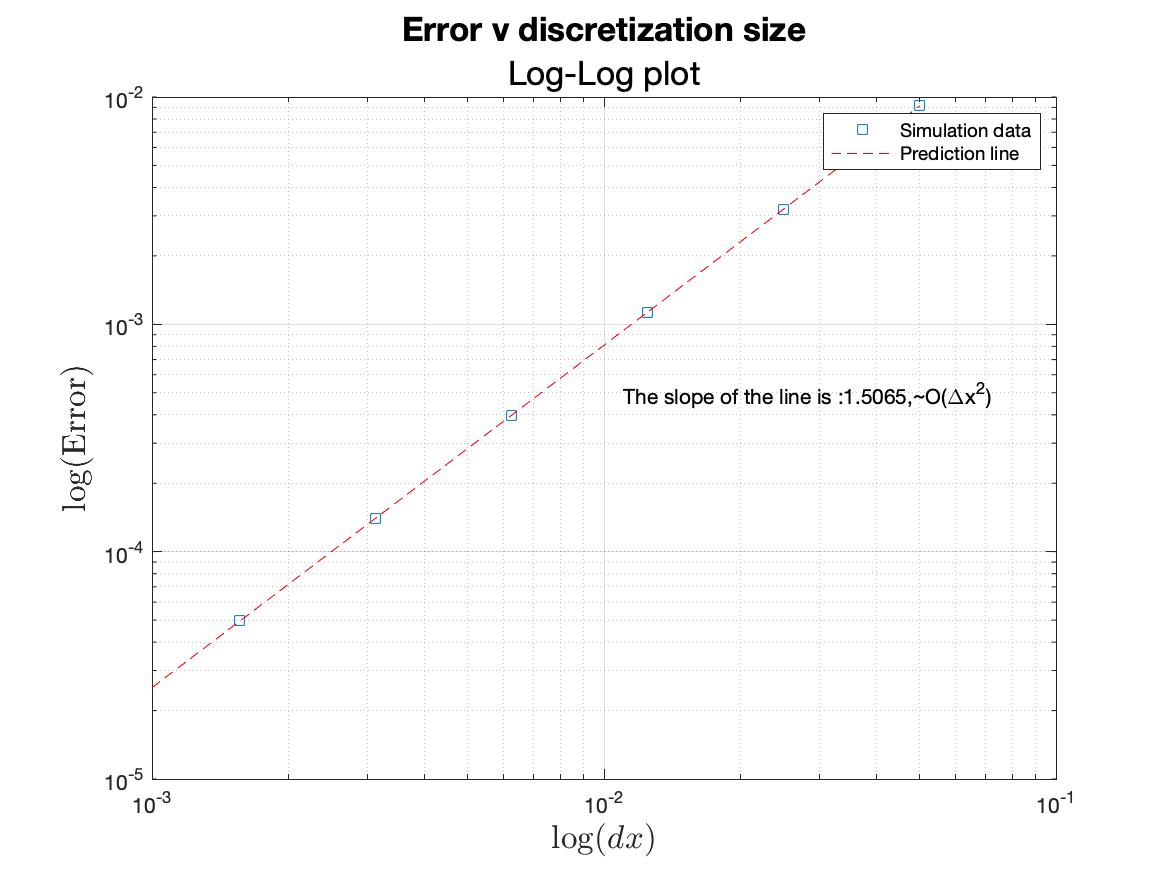
\includegraphics[width=4in]{Err_plot}
\end{center}
\caption{Maximum error (v) Grid refinement}
\label{fig:q3b}
\end{figure}
From Fig~\ref{fig:q3b}, we can deduce that $\max{\text{Error}} \rightarrow 0 \ \text{as} \ \Delta x \rightarrow 0$.
  
  \item {\color{blue}For each of the runs in part (b) determine the computational cost to obtain the approximation at the final time. For example you may use the MATLAB} {\tt tic} {\color{blue}and} {\tt toc} {\color{blue}commands. Discuss the scaling of the computational time with respect to the size of the grid. Produce a} $\log$-$\log$ {\color{blue}plot showing the relation of the computational cost to the number of grid points, and include a reference line indicating the predicted growth in cost.}\\

In the code attached in Listing~3., line 50. and line 60. documents the time taken to calculate the value of $u$ at all the spatial points. The relationship between computational cost with increasing grid refinement  is shown in Fig~\ref{fig:q3c}. The behavior is pretty strange for $N=20$. It makes sense as to why the computational time is increasing as $N$ is increased. With $N \uparrow$, there are more points on the spatial grid, hence the \textbf{for} loop runs for more number of iterations and hence, the rise in computational time is justifiable. But, the reasoning behind why the time taken for $N=20$ is higher than $N=40$ is strange and I am unable to figure it out.
\begin{figure}
\begin{center}
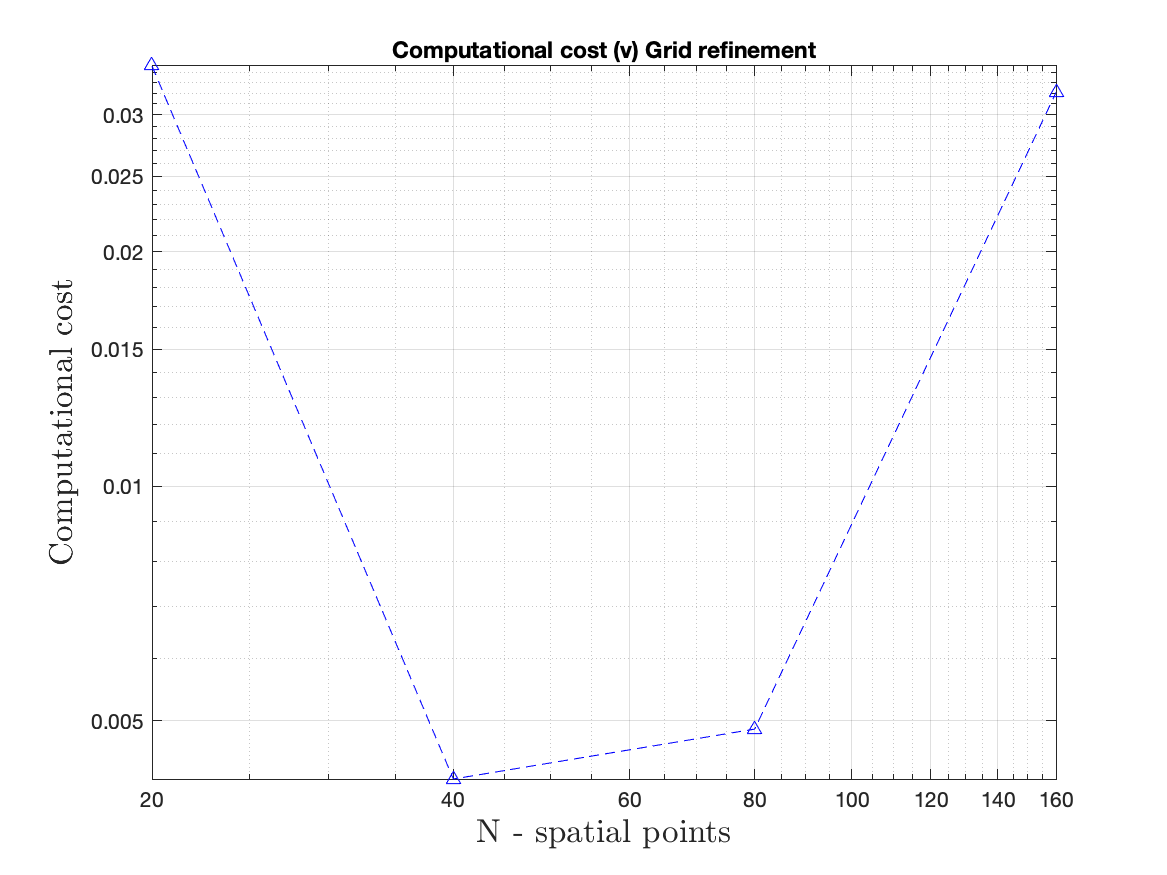
\includegraphics[width=4in]{cost_plot}
\end{center}
\caption{Computational cost (v) Grid refinement}
\label{fig:q3c}
\end{figure}

  \end{enumerate}
  
\end{enumerate}

\end{document}
